\newpage

	Phổ biến nhất, kênh không được sử dụng trực tiếp cho việc truyền tải tín hiệu dải gốc. Tín hiệu dải gốc signal được sử dụng để điều khiển một số thông số của sóng nạp, khiến cho các thông số thay đổi theo sự thay đổi của tín hiệu dải gốc, đây là gọi là tín hiệu tần số. Theo nguyên lý, sóng nạp được chỉnh sửa có thể là bất kỳ dạng sóng nào, miễn là nó phù hợp cho việc truyền tải trung gian và có thể phân biệt được giữa các tín hiệu khác nhau. Thực tế, trong hầu hết các hệ thống giao tiếp số, tín hiệu $sin$ là lựa chọn làm sóng nạp, vì nó đơn giản và dễ tạo và nhận. So với tín hiệu tương tự và tín hiệu số, nguyên lý cơ bản là giống nhau, khác biệt chỉ là trong quá trình tín hiệu tương tự, thông số của sóng nạp được chỉnh sửa liên tục, tại đầu nhận, các thông số của sóng nạp được đánh giá liên tục.


\section{Cơ sở lí thuyết}

    Khi tín hiệu dữ liệu số được truyền bằng phương pháp FM, thì kỹ thuật này được gọi là kỹ thuật dời tần (FSK: Frequency- Shift Keying). Nó được sử dụng rộng rãi vì khả năng chống lại sự mất tầm rất mạnh. FSK được sử dụng để truyền tín hiệu kỹ thuật số với các tần số khác nhau, và tần số của tín hiệu nạp được điều khiển bởi tín hiệu kỹ thuật số cơ sở. Tín hiệu nạp được nhận tại đầu nhận được chuyển đổi thành tín hiệu kỹ thuật số để hoàn thành quá trình truyền thông thông tin. 2FSK là hình thức đơn giản nhất của chuyển dấu chuyển tần số, có thể biểu diễn như sau: \\
	\[S(t) = m_1(t)A\cos(2 \pi f_1 t + \varphi _1) + m_2(t)A\cos(2 \pi f_2 t + \varphi _2) \] \\
	
Mô hình điều chế đa tần số có thể được hình thành bằng cách thêm sóng hình sin với các số khác nhau,tần số và biên độ khác nhau. Ví dụ: \\
	\[ S(t) = 
\begin{array}{cc}
m_1(t)A\cos(2 \pi f_1 t + \varphi _1) & + \\
m_2(t)A\cos(2 \pi f_2 t + \varphi _2) & + \\
m_3(t)A\cos(2 \pi f_3 t + \varphi _3) & + \\
 & \vdots \\
m_m(t)A\cos(2 \pi f_m t + \varphi _m) & +
\end{array}
 \] \\
\subsection{Điều chế}
    Phương pháp điều chế 2-FSK sử dụng các tần số khác nhau của sóng mang để biểu diễn các bit khác nhau (0 hoặc 1) của tín hiệu nhị phân cần mã hóa, nói theo cách khác, sóng tín hiệu truyền đi được tạo ra bằng cách thay đổi tần số của sóng mang.\\
Ta có không gian tín hiệu M:
\[ s_1 = \sqrt{\frac{2}{Tb}} cos(2 \pi f_1 t) \]
\[ s_2 = \sqrt{\frac{2}{Tb}} cos(2 \pi f_2 t) \]

Ta có $f_0 = 1/R_b$. Giải sử sóng mang có cần tần số $f_1, f_2 = kf_0$ , $( k \in Z)$.\\
Ta gán: \\
\begin{itemize}
\item Với giá trị bit $1$ : $\sqrt{\frac{2}{Tb}} cos(2 \pi f_1 t)$
\item Với giá trị bit $0$ : $\sqrt{\frac{2}{Tb}} cos(2 \pi f_2 t)$
\end{itemize}
	
\begin{center}
    \begin{figure}[htp]
    \begin{center}
     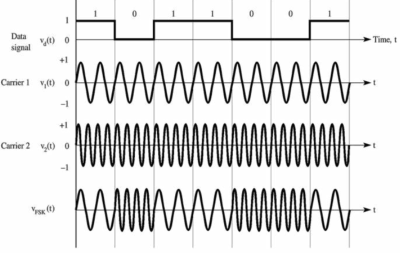
\includegraphics[scale=1]{Img/dieu_che_fsk.png}
    \end{center}
    \caption{Sơ đồ điều chế FSK}
    \label{refhinh1}
    \end{figure}
\end{center}


\subsection{Bộ lọc phối hợp Matched Filter}

Mỗi bộ lọc được đặc trưng bởi đáp ứng xung: $h(t)$ \\
Tín hiệu đầu ra $y(t)$ được xác định bởi tín hiệu đầu vào $x(t)$ và đáp ứng xung như sau:
\[ y(t) = \displaystyle \int_{-\infty}^{\infty} x(\tau)h(t - \tau) d \tau  \]
Theo bài ra ta có: \\
\begin{itemize}
\item Tín hiệu đầu vào là tín hiệu nhận được sau khi điều chế: $p(t)$
\item Đáp ứng xung là $h(t) = b_j(T-t)$
\end{itemize}


Từ đó ta thu được đầu ra của bộ lọc là:
\[ y(t) = \displaystyle \int_{-\infty}^{\infty} p(\tau)h(t - \tau) d \tau =   \displaystyle \int_{-\infty}^{\infty} p(\tau)b_j(T - t + \tau) d \tau \]
Giả thiết lấy mẫu tín hiệu đầu ra tại thời điểm $t = T$
\[ y(t=T) = \displaystyle \int_{-\infty}^{\infty} p(\tau)b_j(\tau) d \tau =  \displaystyle \int_{0}^{T} p(\tau)b_j(\tau) d \tau = p_j\]
\begin{center}
    \begin{figure}[htp]
    \begin{center}
     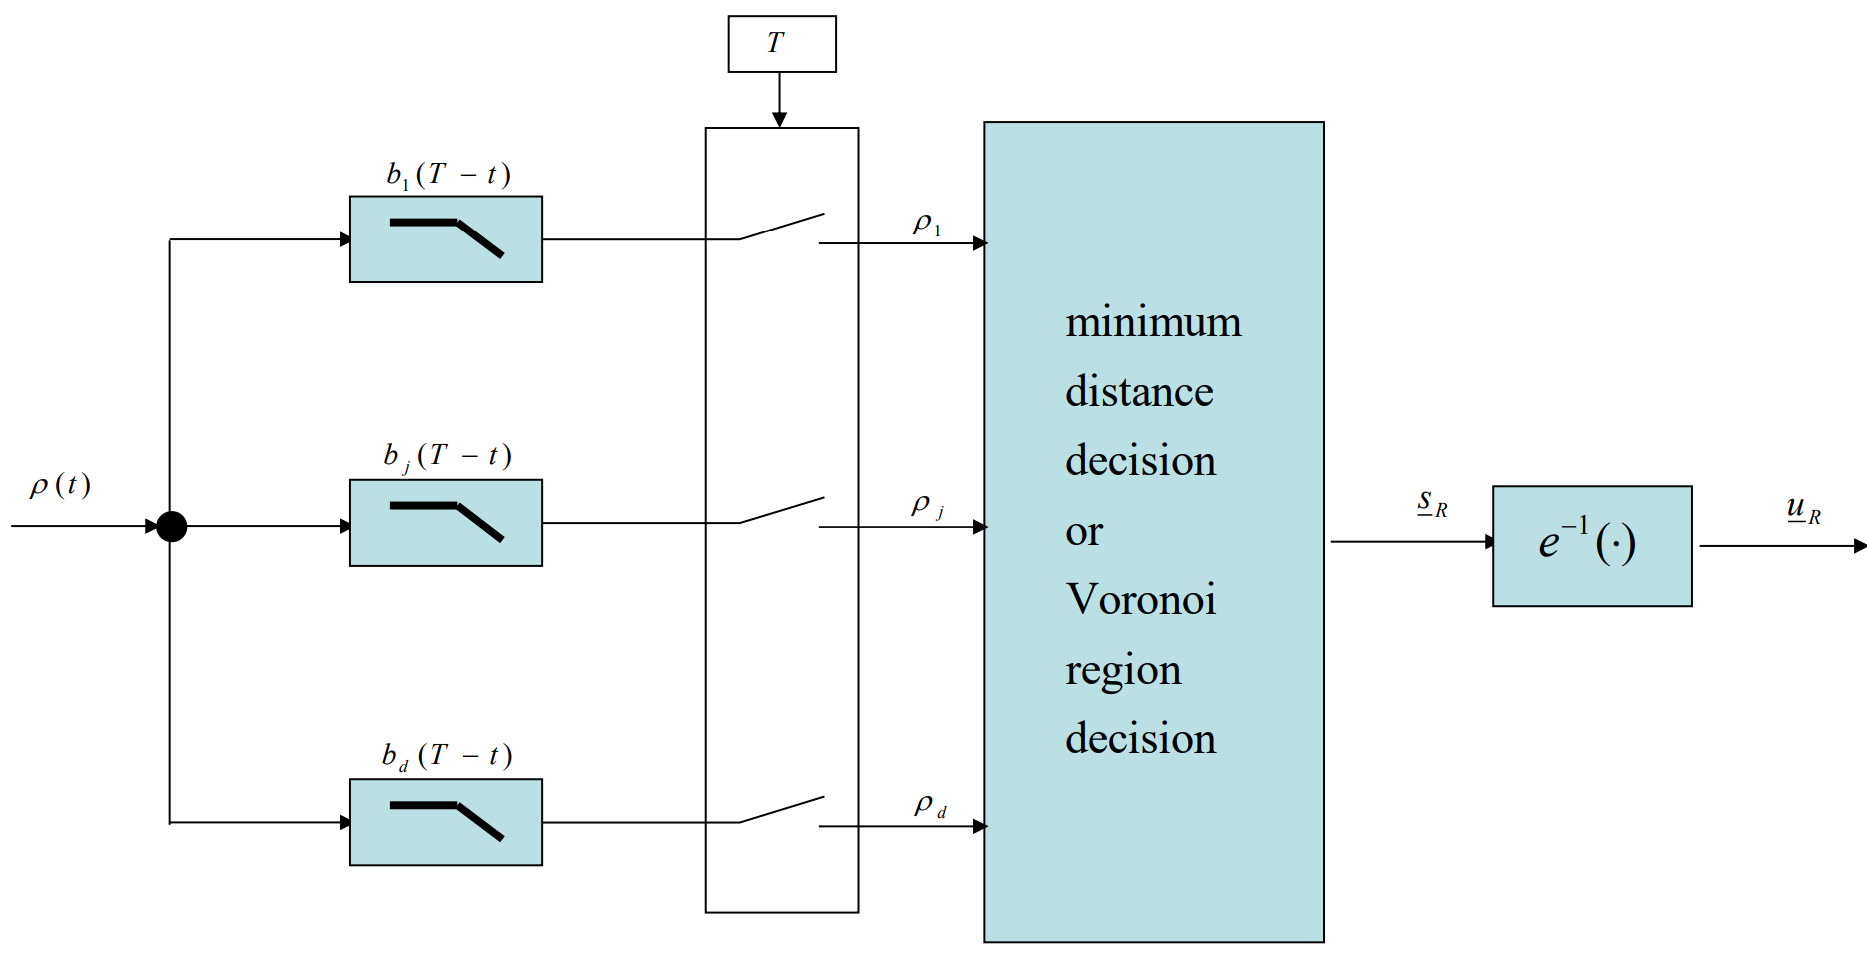
\includegraphics[width=\textwidth]{Img/MF.png}
    \end{center}
    \end{figure}
\end{center}
\subsection{Nguyên lí giải điều chế}
Các bước giải điều chế FSK:
\begin{enumerate}
\item Từ M xây dựng cơ sở trực chuẩn:
\[ b_1(t) = \sqrt{\frac{2}{T}} P_T(t)cos(2 \pi f_1 t) \]
\[ b_2(t) = \sqrt{\frac{2}{T}} P_T(t)cos(2 \pi f_2 t) \]
\item Xây dựng bộ lọc phối hợp Matched Filter (MF)
\item Xác định giá trị đầu ra của bộ lọc tại các thời điểm $t = nT$
\item Tính khoảng cách đến các điểm $s_1$, $s_2$ được biểu diễn trong hệ trục tọa độ trực chuẩn. Nếu khoảng cách nào nhỏ nhất thì quyết định sóng mang này biểu diễn bit nào.



\end{enumerate}


\section{Lập trình với python}
\subsection{Tạo chuỗi bit ngẫu nhiên và tín hiệu xung}
Tạo chuỗi N bit ngẫu nhiên bằng hàm $rantint$ trong python và biểu diễn dưới dạng xung vuông:

\begin{lstlisting}
import random
import numpy as np
import matplotlib.pyplot as plt

def random_bits_array(n):   
    return [random.randint(0, 1) for _ in range(n)]
def message_signal(m,T):  
    t = np.arange(0, T, T/100)
    message = []
    not_message = []
    for i in range(len(m)):
        
        if m[i] == 1:
            m_s = np.ones(len(t))
            invm_s = np.zeros(len(t))
        else:
            m_s = np.zeros(len(t))
            invm_s = np.ones(len(t))
        message.extend(m_s)
        not_message.extend(invm_s)
    return message , not_message
           
N = 8       
Tb = 1       
T = 1*N    
t = np.arange(0, T, T/800)

m = random_bits_array(N)

fig, ax = plt.subplots(2, 1, figsize=(15, 5))
fig.subplots_adjust(hspace=0.5)
ax[0].stem(m)
ax[0].set_title('binary data')
ax[0].set_xlabel('n---->')
ax[0].set_ylabel('b(n)')
message , not_message = message_signal(m,T)
print(len(message), len(not_message))
ax[1].plot(t,message, 'r')
ax[1].set_title('message signal-1')
ax[1].set_xlabel('t---->')
ax[1].set_ylabel('c1(t)')

\end{lstlisting}


\begin{center}
    \begin{figure}[htp]
    \begin{center}
     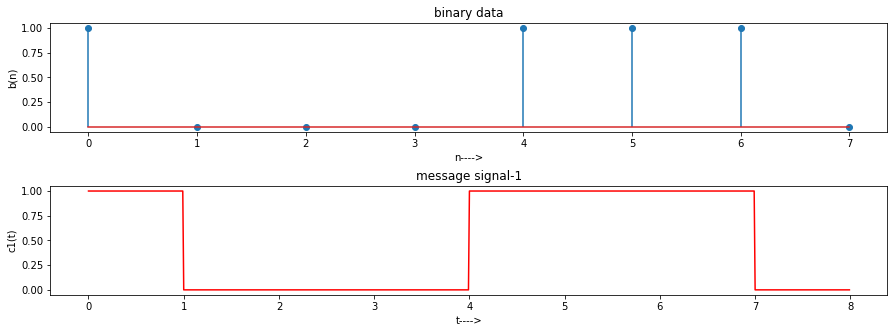
\includegraphics[scale=.5]{Img/binary_signal.png}
    \end{center}
    \caption{Tín hiệu bit và tín hiệu xung}
    \label{refhinh1}
    \end{figure}
\end{center}

\subsection{Tạo tín hiệu sóng mang}
Tạo hai sóng mang cho các tín hiệu tương ứng
\begin{itemize}
\item Với giá trị bit $1$ : $\sqrt{\frac{2}{Tb}} cos(2 \pi f_1 t)$
\item Với giá trị bit $0$ : $\sqrt{\frac{2}{Tb}} cos(2 \pi f_2 t)$
\end{itemize}
\begin{lstlisting}
fc1 = 5
fc2 = 10
c1 = np.sqrt(2/Tb) * np.sin(2 * np.pi * fc1 * t)
c2 = np.sqrt(2/Tb) * np.sin(2 * np.pi * fc2 * t)
fig, ax = plt.subplots(2, 1, figsize=(15, 5))
fig.subplots_adjust(hspace=0.5)
ax[0].plot(t, c1)
ax[0].set_title('carrier signal-1')
ax[0].set_xlabel('t---->')
ax[0].set_ylabel('c1(t)')

ax[1].plot(t, c2)
ax[1].set_title('carrier signal-2')
ax[1].set_xlabel('t---->')
ax[1].set_ylabel('c2(t)')
\end{lstlisting}

\begin{center}
    \begin{figure}[htp]
    \begin{center}
     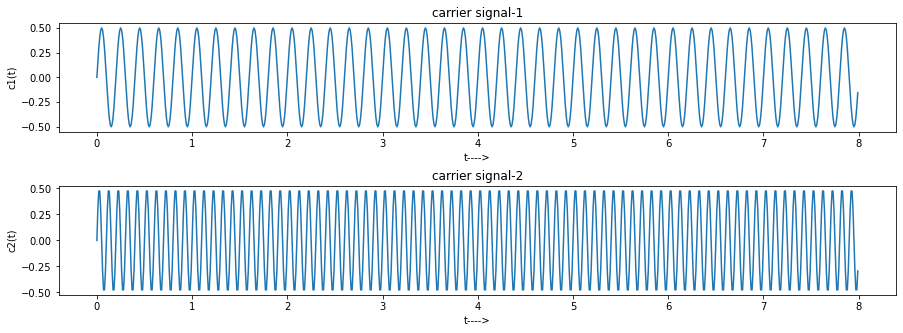
\includegraphics[scale=.5]{Img/carrier_signal.png}
    \end{center}
    \caption{Tín hiệu sóng mang}
    \label{refhinh1}
    \end{figure}
\end{center}

\subsection{Tín kiệu điều chế FSK}
Gán tín hiệu với bit tương ứng. Bit $1$ có tần số $f_1$, bit $0$ có tần số $f_2$.
Gán fsk là mảng chứa giá trị của tín hiệu sau khi điều chế
\begin{lstlisting}
fig, ax = plt.subplots(1, 1, figsize=(15, 3))
def modulation(message_signal,not_message_signal):  
    return message_signal*c1+ not_message*c2
fsk = modulation(message,not_message)
ax.figsize=(15, 5)
ax.plot(t,fsk, 'b')
ax.set_title('FSK signal')
ax.set_xlabel('t---->')
ax.set_ylabel('FSK')
\end{lstlisting}


\begin{center}
    \begin{figure}[htp]
    \begin{center}
     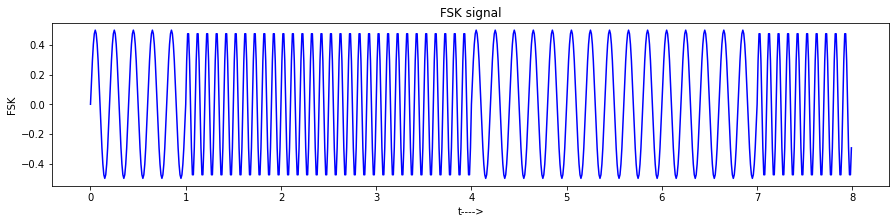
\includegraphics[scale=.5]{Img/modulation.png}
    \end{center}
    \caption{Tín hiệu điều chế}
    \label{refhinh1}
    \end{figure}
\end{center}

\subsection{Giải điều chế}
	
	
\begin{lstlisting}
fig, ax = plt.subplots(1, 1, figsize=(15, 3))
def demodulation(fsk,N):
    start = 0
    end = 99
    demod = np.zeros(N)
    for i in range(N):
        x1 = np.sum(c1[start:end] * fsk[start:end])
        x2 = np.sum(c2[start:end] * fsk[start:end])
        x = x1 - x2
        if x > 0:
            demod[i] = 1
        else:
            demod[i] = 0
        start += 100
        end += 100
    return demod
demod = demodulation(fsk,N)
ax.stem(demod)
ax.set_title("Demodulated data")
ax.set_xlabel("n---->")
ax.set_ylabel("b(n)")
\end{lstlisting}

\begin{center}
    \begin{figure}[htp]
    \begin{center}
     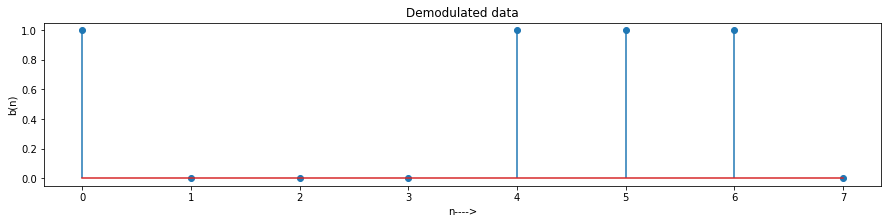
\includegraphics[scale=.5]{Img/demodulation}
    \end{center}
    \caption{Giải điều chế}
    \label{refhinh1}
    \end{figure}
\end{center}

\subsection{Điều chế và giải điều chế FSK dưới tác động của nhiễu Gausian}
Dùng hàm random.random trong python để tạo phân bố chuẩn Gauss
\begin{lstlisting}
def white_noise(rho, sr, n, mu=0):
    sigma = rho * np.sqrt(sr/2)
    noise = np.random.normal(mu, sigma, n)
    return noise
gauss = fsk + white_noise(1,1,800)
fig, ax = plt.subplots(1, 1, figsize=(15, 5))
ax.plot(gauss, 'b')
ax.set_title('FSK signal')
ax.set_xlabel('t---->')
ax.set_ylabel('FSK')

\end{lstlisting}
\begin{center}
    \begin{figure}[htp]
    \begin{center}
     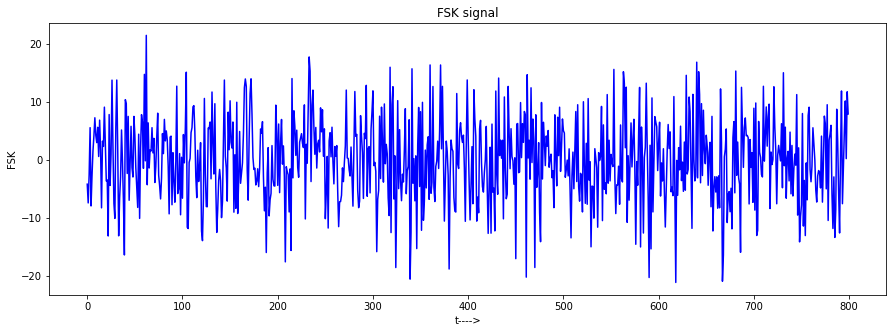
\includegraphics[scale=.5]{Img/add_gauss_signal.png}
    \end{center}
    \caption{Tín hiệu thêm nhiễu Gauss}
    \label{refhinh1}
    \end{figure}
\end{center}
\newpage
\section{Tính xác suất lỗi bit}
Chiếu hai tín hiệu nên không gian trực chuẩn ta có:
\[ M = \{ s_1(1,0), s_2(0,1) \} \]
Từ đó ta có vùng Voronoi được định nghĩa như sau:
\[ V(s_1) = \{  p = (p_1,p_2), p_1 \ge p_2 \} \]
\[ V(s_2) = \{  p = (p_1,p_2), p_2>p_1 \} \]
Ta có:
\begin{equation}
	P_s(e) = \frac{1}{2} (P_s(e|s_T = s1) + P_s(e|s_T = s_2)  
\end{equation}
 
Ta cần tính:
\[  P_s(e|s_T = s_1) = P(p \in s_2 | s_T = s_1) = P(p_2 > p_1 | s_T = s_1)\]
Mà $ p_1 = s_1 + n_1 $, $ p_2 = s_2 + n_2  $ và $s_1 = s_2 = 1$ suy ra:
\[ P_s(e|s_T = s_1) = P(n_2 > n_1) = P(n_2 - n_1 > 0)\]
\[ \rightarrow P_s(e|s_T = s_1) = \frac{1}{2} erfc(0) \]
Tương tụ ta có 
$P_s(e|s_T = s_2) = \frac{1}{2} erfc(0) $ \\
Thay vào (1) ta có $P_s(e) = \frac{1}{2} erfc(0)$

Vậy xác suất lỗi bit trong AWGN là: $P_s(e) = \frac{1}{2} erfc(0)$
